\newpage

\section{Experimenty}
\label{experiments}
Počas zostrojovania neurónovej siete sme vykonali niekoľko experimentov, týkali sa hlavne konfigurácie siete, rôznych aktivačných funkcií, optimizérov a veľkosti datasetu pri trénovaní. Väčšie experimenty sú popísané v častiach \ref{val_vs_noval} a \ref{dropout_vs_nodropout}, zistenia z tých menších sú zhrnuté nasledovne:

\begin{itemize}
	\item najlepšie sa sieť učí, keď dostane naraz celý trénovací dataset, nie len jeho časti
	\item pridanie ďalších plne prepojených vrstiev predikcie zhoršilo
	\item pridanie viacerých konvolučných vrstiev nemalo prakticky žiadny vplyv na predikcie
	\item použitím štandardnej ReLU aktivačnej funkcie dosahovala chyba predikcie enormné hodnoty, bez ohľadu na rýchlosť učenia a použitý optimizér (Adam, Gradient descent, ...)
	\item aktivačná funkcia Sigmoid v kombinácii s Ftrl optimizérom, ktorého rýchlosť učenia bola 0.2, dávala najnižšiu chybu predikcií
\end{itemize}

Na základe vyššie uvedeného sme teda do ďalších experimentov pokračovali s modelom neurónovej siete, kde bola aktivačná funkcia Sigmoid, Ftrl optimizér, rýchlosť učenia 0.2 a rovnaký počet konvolučných a plne prepojených vrstiev ako v zobrazenom modeli v časti \ref{navrh}.

\subsection{Model s validáciou vs. model bez validácie}
\label{val_vs_noval}
Nakoľko máme dosť malý dataset, experimentovali sme s modelom, kde nebola použitá validácia a dáta pre ňu určené boli pridelené k trénovacím dátam. Výsledok však dosiahol iba zhoršenie priemernej chyby predikcie o 0.001. Tréning bez validácie končil v momente, keď chyba na tréningových dátach začala rásť, s validáciou končil až keď začala rásť na validačných dátach. To vyústilo vo viac ako 2x dlhší tréning, ako môžete vidieť na obrázku \ref{validation_graph}. 

	\begin{figure}[H]
			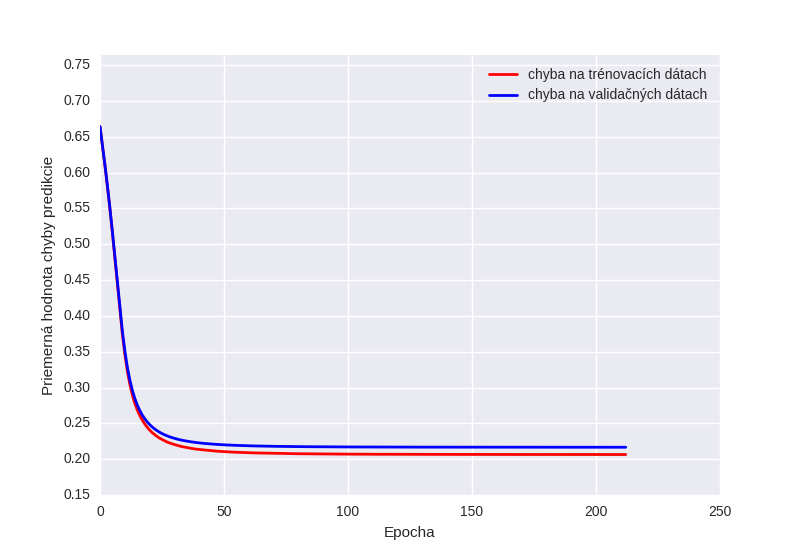
\includegraphics[scale=0.33]{train+val.png}
			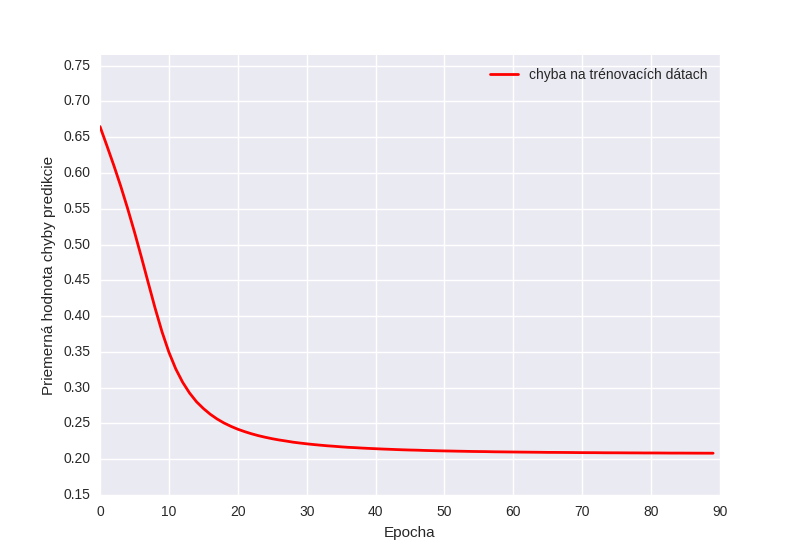
\includegraphics[scale=0.33]{train.png}
		\caption[Trénovanie s validáciou vs. trénovanie bez validácie]{Grafy poklesu chyby pri jednotlivých trénovaniach, vľavo trénovanie s validáciou, vpravo bez nej}\label{validation_graph}
	\end{figure}
	
Chyba na natrénovanom modeli bez validácia bola na testovacích dátach 0.2088, na trénovacích 0.2061. Na natrénovanom modeli s validáciou bola chyba na testovacích dátach 0.2078, na validačných 0.2166 a na trénovacích 0.2066. Takže zlepšenie bolo síce minimálne, ale stále badateľné. Hlavný dôvod, prečo validácia nemala až taký účinok, je malé množstvo dát. 

\subsection{Model s vrstvou výpadku vs. model bez vrstvy výpadku}
\label{model_graph}
\label{dropout_vs_nodropout}
Ďalšiu konfiguračnú zmenu, s ktorej implementáciou sme experimentovali, bolo pridanie vrstvy výpadku. Výsledok bol však len ten, že sieť sa dokázala naučiť to isté za rýchlejší čas, predikcie sa ale nezlepšili, ako je vidieť na nasledujúcich grafoch na obrázku \ref{dropout}. 

	\begin{figure}[H]
		
		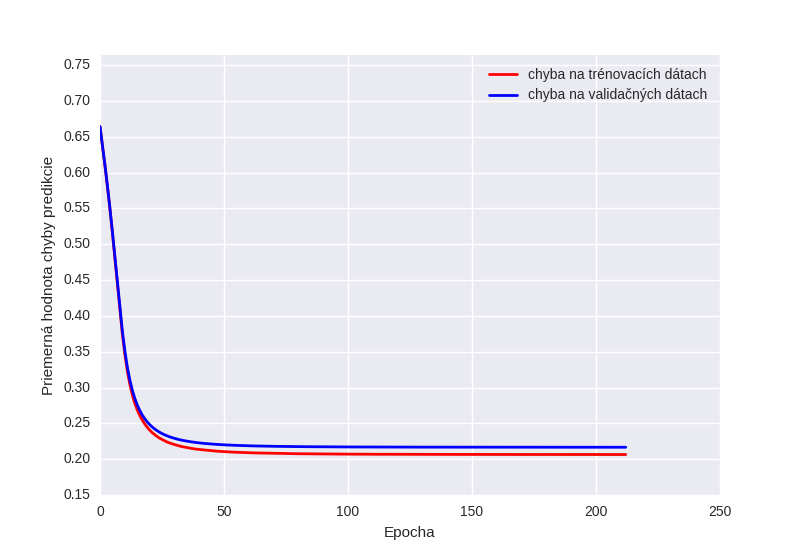
\includegraphics[scale=0.33]{train+val.png}
		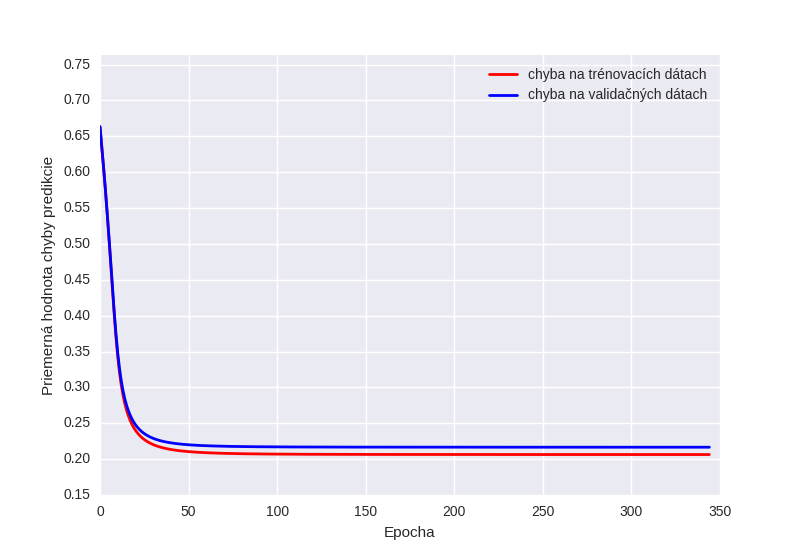
\includegraphics[scale=0.33]{without_dropout.png}
		\caption[Model s vrstvou výpadku vs. bez nej]{Grafy poklesu chyby pri jednotlivých trénovaniach, vľavo model s vrstvou výpadku, vpravo bez nej}\label{dropout}
	\end{figure}
	
